\documentclass[main]{subfiles}

\begin{document}

\chapter{Long reads assembly tools state of the art}\label{chapter:sota}

In this chapter we present some long-read assembly tools we select this tools because method and algorithm used in it was representative how other tools work in addition, these tools are recognized by the community for their quality.

\section{A Pipeline with correction \canu} \label{section:sota:canu}

\canu is based on \toolsname{Celera} \cite{celera_first, celera_second}, we can split the \canu pipeline in three step, correction, trimming, assembly, before each step \canu search overlap between reads.

\paragraph{Overlapping}

To avoid all versus all alignment \mhap try to estimate which read share a common part by estimate a Jaccard distance between the set of \kmers of two reads. The Jaccard distance, present in equation \ref{sota:equ:jaccard_dist} evaluate the distance between two set by divide the intersection of set by union of set.

\begin{equation}
J_{\delta}(A,B) = 1 - J(A,B) = 1 -  J(A,B) = 1 - \frac{|A \cap B|}{|A \cup B|}
\label{sota:equ:jaccard_dist}
\end{equation}

Enumerate all \kmers of each reads and compute intersection and union of each set take many times. \mhap select a subset of \kmers to represent the read and compute a mash distance \cite{mash_distance} see equation \ref{sota:equ:mash_dist_def} 

\begin{equation}
J(A,B) = \frac{|A \cap B|}{|A \cup B|} \approx \frac{|S(A \cup B) \cap S(A) \cap S(B)|}{|S(A \cup B)|}
\label{sota:equ:mash_dist_def}
\end{equation}

$S(A)$ is a \kmers set compose by $s$ first \kmers of set $A$. \citeauthor{mash_distance} evaluate the error between mash distance and jaccard distance was in $\mathcal{O}(\frac{1}{\sqrt{s}})$, by default in \mhap $s=512$ so the error was smaller than 0.05.

In \mhap order \kmer with a \texttt{tf-idf} score, see equation \ref{sota:equ:tf_idf_def}. The \texttt{tf-idf} score come for text search domain, try to say if this term is specific to this document. \texttt{tf} for term frequency indicate if the term was present many times in document, $n_{i,j}$ how many time the term $i$ was present in document $j$ divide by the number of term in document $j$. \texttt{idf} for inverse document frequency evaluate if the term was present in many document or just in some document, $|\mathcal{D}|$ the number of document in dataset divide by $|\{d_{j}:t_{i}\in d_{j}\}|$ the number of document where the term $i$ was present.

\begin{equation}
\mathrm{tf-idf_{i,j}} = \mathrm{tf_{i,j}} \cdot \mathrm{idf_{i}} = \frac{n_{i,j}}{\sum_{k}n_{k,j}} \cdot \log{\frac  {|\mathcal{D}|}{|\{d_{j}:t_{i}\in d_{j}\}|}}
\label{sota:equ:tf_idf_def}
\end{equation}

In \mhap term was \kmer and document was read, this technique permit to reduce the number of kmer in set and keep kmer specific to a read. If two read share specific kmer they probably share a common part.

If two reads have a small mash distance \mhap compare the position of each \kmer in reads to determinate the overlap position.

The size of kmer was very important to if k is too large many kmer contains error the size of intersection was reduce and \mhap can miss overlap. Moreover size of sketch have a huge impact if it's to small the read was sub-sample if it's to large compute mash distance take more time, but with long-reads dataset the length of reads can be very different choose a good sketch size for this type of data isn't easy.

\paragraph{Correction}

In \canu correction was performed by a part of \toolsname{FALCON} \cite{falcon}, \toolsname{falcon\_sense}. In this section we didn't present in details how \toolsname{falcon\_sense} work but only the main idea.

Some correction tools as \toolsname{falcon\_sense} use a Partial Order Alignment (POA) (introduce in \cite{poa}) to perform long read correction. For each read \texttt{$R_1$} we recruit all read share an overlap with him, and perform an exact alignment with him. This alignment was use to build a POA graph, in POA graph each base was a node and a direct edge was create between two base if the first base was before the second one in an alignment. If an edge was present in two alignment her weight was increment. After all alignment was add in the POA graph, we search weighed path in this graph, and follow to reconstruct the corrected sequence. An example of POA graph construction was present in figure \ref{sota:fig:canu:correction}

\begin{figure}[ht]
    \centering
    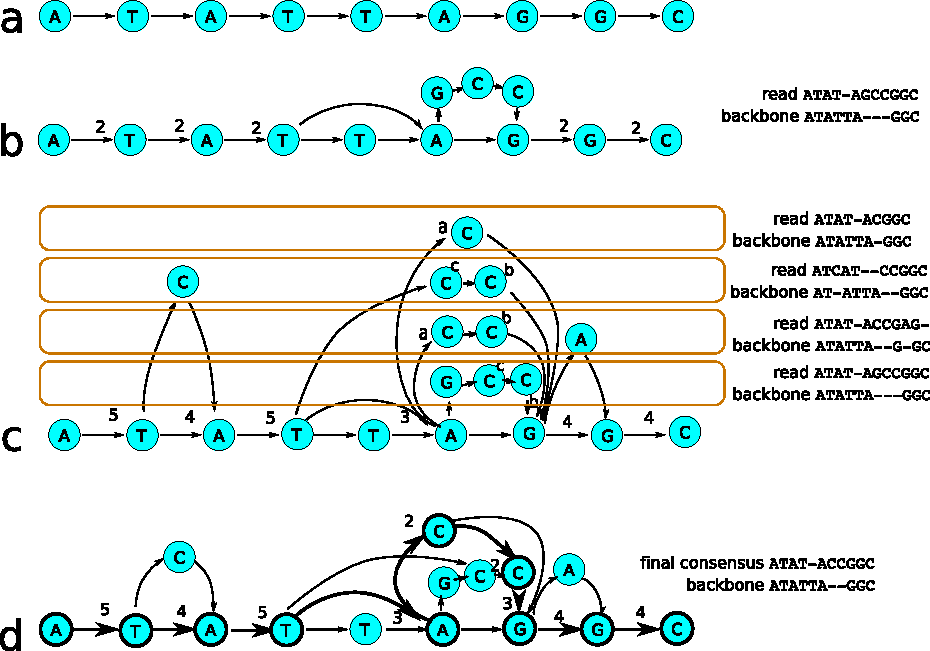
\includegraphics[width=\textwidth]{state_of_the_art/images/POA_explain.pdf}
    \caption{Sequence need to be correct was represent as a graph, each base was a node and if a base is follow by another an directed edge was build. (b) was the representation of sequence \texttt{ATATTAGGC} (call backbone in this figure), (b) We add the result of alignment of one read in the graph, number upper than edge was her weigth if and edge exist in some 3 alignment her weight was egal to 3, (c) We add all other alignment in the graph, (d) the bold path was choose a the correct path because it was supported by more alignment. This figure was originaly present in Supplementary material of \hgap \cite{hgap}}
    \label{sota:fig:canu:correction}
\end{figure}

\paragraph{Trimming}

The trimming step will remove the parts of the reads that are not supported by the other reads, see Figure \ref{sota:fig:canu:trimming}. For each reads we will analyze its coverage curve and remove the parts of the reads that are not sufficiently covered, for trimming \canu use an homemade tools.

\begin{figure}[ht]
    \centering
    \subfile{state_of_the_art/tikz/trimming.tex}
    \caption{Black line was a reads, the \canu trimming step keep only the blue part of read $R_0$, part covered by other read.}
    \label{sota:fig:canu:trimming}
\end{figure}

\paragraph{Assembly}

\canu assembly step is based on \OLC paradigm, with some specificity \canu build a Best Overlap Graph (BOG) for each not contained read only two overlap are kept in the graph, the best overlap for each read extremity, in \canu the best overlap was the longest overlap. After this graph construction step performed, some clean step was run, remove tips (a read with no sucessor), little buble.

This BOG was used as a scaffold to generate assembly, by remapping read against this scaffold, \canu try to detect repetition, larger than read not show in BOG as loop, and to call read to build a consensus after. Each simple path in BOG was used to build a contig. 

By remapping reads on the BOG \canu can build a consensus and detect repetition didn't observe in graph. BOG was an aggressive strategy to avoid transitive edge and reduce graph size but they can mask an edge denote a repetition this check was required to.


\section{Pipeline without correction \miniasm} \label{section:sota:miniasm}

\minimap and \miniasm was an assembly pipeline proposed in \cite{miniasm_minimap} and \cite{minimap2}, the main purpose of this pipeline is to demonstrate we can perform a long read assembly without correct long read before.

\subsection{\minimap}

Main idea to \minimap (similar to \mhap) is we can represent a read as a set of some minimal kmer, and if two read share same succession of minimal kmer we can suppose this two read share an overlap.

A minimal kmer is a the kmer for a set of consecutive kmer than minimize her score, the score function was the same during all analyse and for the same set of consecutive kmer the same kmer was the minimizer. Moreover a kmer can be minimizer of some consecutive set of kmer, if no other kmer with lowest score come in window. 

\begin{figure}[ht]
    \centering
    \subfile{state_of_the_art/tikz/minimizer.tex}
    \caption{The red kmer was the minimizer of the read box and the blue kmer was the minimizer of the blue box.}
    \label{sota:fig:miniasm:minimizer}
\end{figure}

The minimal kmer can represent many other read, this technique can be compare to a loosly compression.

\minimap build an index where each minimizer are associate to reads where minimizer is present and position of this minimizer in reads.

With this index \minimap can collect position of similar minimizer between two reads, with this collection of position \minimap search the largest co-linear match, a succession of similar minimizer in each reads with coherent position, same order of minimizer and similar distance between each minimizer. Figure \ref{sota:fig:miniasm:mapping} show an overview of a overlap of two reads in \minimap.

\begin{figure}[ht]
    \centering
    \subfile{state_of_the_art/tikz/minimap.tex}
    \caption{$Read_A$ and $Read_B$ was represent by black arrow. Common minimizer of $Read_A$ and $Read_B$ was represent by blue and red arrow respectively. Green arrow was a co-linear chain, purple arrow was another co-linear chain, black arrow didn't participate to a co-linear chain.}
    \label{sota:fig:miniasm:mapping}
\end{figure}

\minimap report overlap where the number of match is sufficient (upper than a threshold) and  total length of putative overlap was sufficient. 

\subsection{\miniasm}

\miniasm didn't perform correction but they didn't take all information from reads and overlap, some filtering operation was performed.

For each read \miniasm perform coverage analysis of reads based on mappings identify by \minimap, by default only the longest part of reads with a coverage upper than three are kept. \minimap report for each read, read length, position of first and last kmer, number of bases in kmer exact match,  and a mapping quality and some option field in SAM like format can be present too.

\begin{figure}[ht]
    \centering
    \subfile{state_of_the_art/tikz/miniasm_overlap.tex}
    \caption{\miniasm classify overlap in three type of dovetail, internal match and containment overlap. Black grey region correspond to part of read between first and last minimizer. Light grey region was called overhang region, it's out of minimizer range. If overhang was large compare to overlap region we can supects this overlap isn't a true overlap.}
    \label{sota:fig:miniasm:ovl_classification}
\end{figure}

Each overlap was classified, in three category:
\begin{itemize}
    \item internal match, this type of overlap probably correspond to a repetition smaller than reads length
    \item containment, a read of this overlap was contains in the other read it's same sequence
    \item dovetails, it's a end-to-end overlap
\end{itemize}
Figure \ref{sota:fig:miniasm:ovl_classification} show some exemple of this overlap. Containment read was removed, only dovetail overlap was used to build overlap graph. Tips, small bubble and transitive edge was removed after this step \miniasm take each simple path and concatenate substring of read between begins and the first position of overlap.

\miniasm was design to work on uncorrected read and didn't perform a consensus step so contigs generate by \miniasm contains many error and can't be used directly. We can run \minimap \miniasm pipeline with corrected read and a polishing tools on contig generate by \miniasm. 

\toolsname{Ra}\cite{Ra} was a tools create to replace \miniasm in \minimap \miniasm pipeline. \toolsname{Ra} use an analysis of coverage curve of each reads to trimm not supported region, detect chimera and repeat region. Overlap on region marked as repeat are marked in string graph and not trusted. \toolsname{Ra} perform a real consensus step and run many polishing step with \toolsname{Racon}.

\section{\DBG and \DBG like long reads assembly approach} \label{section:sota:wtdbg}

The \DBG approach was not the preferred one for the assembly of long reads because :
\begin{itemize}
    \item reads contain a high error rate and therefore found error-free kmers was hard, this error can lead to expand size of graph and or mis-connection between part of graph.
    \item size of kmer was generaly lower than 100 base and manage larger kmer was hard without usage of many memory, moreover \DBG can't manage repetition larger kmer.
\end{itemize}

If we use \DBG naively for long read assembly, we can mis the main advantage of long-reads her length.

Some \flye and \wtdbg use \DBG approach with some modification to adapt this idea to long-read assembly.

\subsection{\flye}

\flye\cite{Flye} was based on \abruijn\cite{abruijn} assembly tools. \abruijn didn't use a \DBG but a similar concept a \abreviation{ABG} (for A-Bruijn Graphs), in place of use a set of kmers as node \abreviation{ABG} use a set of chosen kmers, in place of build an edge between each kmer they share a k-1 overlap they use \abreviation{ABG} build an edge with a weight equal to the distance of kmer in the original string between without create transitive edge.

To build the chosen kmers set, \abruijn select kmers present many times in dataset this kmers was called in many tools \textit{solid} kmers. The more a kmers is present in the dataset, the more sure you may be that this kmers does not contain a sequencing error, if I sequence my genome with 40x I can hope see kmer, not include in a repetition, 40 times. Because when we sequence at 40x we didn't really read each base 40 times and when a sequence error appear we lost an occurrence of the kmers where this base was present, choose the number of times a kmer need to be present in dataset to be \textit{solid} was an hard task.

This modification help to clean sequencing error, but reduce the set of kmer fragment \DBG graphes it's why \abreviation{ABG} create edge not only when kmers share k-1 overlap. 

During the \abreviation{ABG} construction \abruijn store wich read generate wich graph path, this structure was usefull to found speedly overlap between reads. To build contigs \abruijn take a read $R_1$ found all overlap with help of \abreviation{ABG} if this local overlap graph didn't denote a fork, we have one read without successor and all reads have path in graph to this read, \abruijn extend the contig.

\abruijn can be rugly resume as mix of all assembly strategy, use \DBG to found overlap between read, build contigs by extension like \textit{greedy} technique but use \OLC to check they aren't integrate a repetition and a potential missassembly in contigs.

\flye was build on top of \abruijn by building a repetition graph of \abruijn contig, to try to solve it.

\subsection{\wtdbg}

\wtdbg use a \DBG approch to solve long-read assembly, isn't realy a \DBG but a "Fuzzy-Brujin graph" (\abreviation{FDBG}). To build this graph \wtdbg split read in bin with a fixed size (256 base pairs) and they store kmer present in each bin in a hash table.
To find overlap between reads wtdg2 use an hash table to compare the kmer composition between each reads and perform an exact alignment between each bin of reads. 

After this alignment step \wtdbg keep only in memory wich bin are align to which bin, and they build a k-bins each k-bins is a sequence of k successive bin in a read, \wtdbg can infer if two k-bins overlap if some bin in this two k-bins share an ovelap.

A group of k-bins are a node of \abreviation{FDBG}, \wtdbg build an edge between two node if a k-bins in each node are succesive in a read, after some cleanning step (pops bubbles, tips cleanning) \wtdbg build a consensus sequence with each simple path in \abreviation{FDBG}.

\onlyinsubfile{
\bibliographystyle{plainnat}
\bibliography{main}
\addcontentsline{toc}{chapter}{Bibliography}
}

\end{document}